\documentclass[12pt]{article}


%%%%%%%%%%%%%%%%%%%%%%%%
% Imports
%%%%%%%%%%%%%%%%%%%%%%%%
\usepackage[utf8]{inputenc}
\usepackage[italian]{babel}
\usepackage{listings}
\usepackage{color}
\usepackage{hyperref} % Extensive support for hypertext in LATEX (https://ctan.org/pkg/hyperref)
\usepackage{csquotes}
\usepackage[title]{appendix}
\usepackage{graphicx} % Enhanced support for graphics (https://ctan.org/pkg/graphicx)
\usepackage{framed} % Framed or shaded regions that can break across pages (https://ctan.org/pkg/framed)
\usepackage[acronyms,style=altlist,nopostdot]{glossaries}
\usepackage[font=small,labelfont=bf,tableposition=top]{caption}
\usepackage[style=numeric,useprefix,hyperref,backend=bibtex,sorting=none]{biblatex} % Sophisticated Bibliographies in LATEX (https://ctan.org/pkg/biblatex)
\usepackage{subfig}
\usepackage{forest} % Drat tree like data structures (https://ctan.org/pkg/forest)
\usepackage{amssymb}

%%%%%%%%%%%%%%%%%%%%%%%%
% Settings
%%%%%%%%%%%%%%%%%%%%%%%%
\renewcommand*{\lstlistingname}{Cod.}
\renewcommand*{\figureautorefname}{Fig.}
\renewcommand*{\chapterautorefname}{Cap.}
\renewcommand*{\sectionautorefname}{Sez.}
\renewcommand*{\subsectionautorefname}{Sub-sez.}
\graphicspath{ {./img/} } % Base image path

%%%%%%%%%%%%%%%%%%%%%%%%
% References
%%%%%%%%%%%%%%%%%%%%%%%%
\addbibresource{resources.bib} %Import the bibliography file

%%%%%%%%%%%%%%%%%%%%%%%%
% Glossary
%%%%%%%%%%%%%%%%%%%%%%%%
\makeglossaries
\loadglsentries{glossary}

%%%%%%%%%%%%%%%%%%%%%%%%
% Tamarin language
%%%%%%%%%%%%%%%%%%%%%%%%
\definecolor{darkGreen}{HTML}{6A9955}
\definecolor{lightYellow}{HTML}{DCDCAA}
\definecolor{purple}{HTML}{C586C0}
\definecolor{darkRed}{HTML}{D16969}
\lstdefinelanguage{spthy}{
    keywords={equations, functions, builtins, protocol, property, theory, begin, end, subsection, section, text, rule, pb, lts, exists-trace, all-traces, enable, assertions, modulo, default_rules, anb-proto, in, let, Fresh, fresh, Public, public},
    keywordstyle=\color{blue}\bfseries,
    keywords=[2]{aenc, adec, senc, sdec, sign, verify, Eq, eq, hashing, signing, revealing-signing, diffie-hellman, symmetric-encryption, asymmetric-encryption, multiset, bilinear-pairing, h, H, sk, pk, Fr, In, Out, IN, OUT},
    keywordstyle=[2]\color{darkRed}\bfseries,
    keywords=[3]{in, let, begin, end},
    keywordstyle=[3]\color{lightYellow}\bfseries,
    keywords=[4]{axiom, restriction, lemma, sources, use_induction, reuse, hide_lemma, left, right, builtins, protocol, property, subsection, section, text, theory},
    keywordstyle=[4]\color{purple}\bfseries,
    keywords=[5]{F, T, All, Ex, not, &, ==>, =, ==, <, >},
    keywordstyle=[5]\color{red}\bfseries,
    keywords=[6]{<-, <->, !=, <=, >=, --[, ]->, [, ], -->},
    keywordstyle=[6]\color{black}\bfseries,
    identifierstyle=\color{black},
    sensitive=true,
    comment=[l]{//},
    morecomment=[s]{/*}{*/},
    commentstyle=\color{darkGreen}\ttfamily,
    escapeinside={\%*}{*)},
    inputencoding=utf8,
    extendedchars=true,
    literate={á}{{\'a}}1 {ò}{{\'o}}1 {è}{{\'e}}1,
}
\lstset{
    language=spthy,
    extendedchars=true,
    basicstyle=\ttfamily\footnotesize,
    showstringspaces=false,
    showspaces=false,
    tabsize=2,
    breaklines=true,
    showtabs=false
}


%%%%%%%%%%%%%%%%%%%%%%%%
% Begin document
%%%%%%%%%%%%%%%%%%%%%%%%
\begin{document}

% Metadata
\title{Analisi formale di MTProto}
\author{Ernesto Casablanca}
\date{\today}
\makeatletter

% Title page
\begin{titlepage}
    \centering
    
\includegraphics[width=2.434cm,height=2.565cm]{university_logo.png}

    \bigskip

    {\Large \textbf{UNIVERSITÀ DEGLI STUDI DI CATANIA}}

    {\scshape
        \large
        Dipartimento di Matematica e Informatica
    }

    \bigskip

    \hrule

    \bigskip
    \bigskip
    \bigskip
    \bigskip

    {\itshape
        \large
        \@author
        \par}

    \bigskip
    \bigskip
    \bigskip
    \bigskip

    {\centering
        \Large
        \@title
        \par}
    \vspace{5mm}
    {\centering
        Formal analysis of MTProto
        \par}

    \bigskip
    \bigskip
    \bigskip
    \bigskip
    \bigskip
    \bigskip

    \begin{minipage}[b]{8 cm}
        \hrule
        \bigskip
        {\centering\scshape
            Relazione progetto di Computer Security
            \par}
        \bigskip
        \hrule
    \end{minipage}

    \bigskip
    \bigskip
    \bigskip
    \bigskip
    \bigskip
    \bigskip
    \bigskip
    \bigskip
    \bigskip
    \bigskip
    \bigskip

    {\raggedleft
        Professore: Giampaolo Bella
        \par}

    \bigskip
    \bigskip
    \bigskip
    \bigskip

    \vfill

    \hrule

    \bigskip

    {\centering
        Anno Accademico 2021 - 2022
        \par}

\end{titlepage}

% Index
\tableofcontents
\newpage

% Abstract
\begin{abstract}
    \gls{tamarin} è un potente tool utilizzato per effettuare l'analisi formale assistita di protocolli di sicurezza.
    In generale, il risultato può essere ottenuto in automatico dallo strumento.
    Però, poiché il tipo di analisi formale è indecidibile, può capitare che il prover non si arresti.
    Bisogna quindi intervenire manualmente, utilizzando la modalità interattiva. \\
    Utilizzare \gls{tamarin} permette di ottenere una maggiore sicurezza a proposito delle garanzie che un determinato protocollo è in grado di offrire, o, al contrario, ne evidenzia le criticità.
    È per questo che \gls{tamarin} impiegato spesso in ambiti in cui assicurarsi che il protocollo offra effettivamente le proprietà di sicurezza desiderate.
\end{abstract}

\pagebreak

% Tamarin
\section{Tamarin prover}

\subsection{Input}

In questa introduzione ci si soffermerà di una breve descrizione sul funzionamento di \gls{tamarin}. \\
\gls{tamarin} è uno strumento in grado di effettuare la modellazione simbolica e, a partire da questa, l'analisi formale di protocolli di sicurezza.
Per poter avviare una dimostrazione, bisogna fornire in input
\begin{itemize}
    \item il modello che rappresenta fedelmente e correttamente il protocollo
    \item le libertà concesse all'avversario
    \item le proprietà di sicurezza che si desidera assicurare
\end{itemize}
Quello che il tool cercherà di fare è dimostrare se le proprietà indicate sono verificate dal protocollo o, in caso contrario, un attacco che le comprometta.

\subsection{Multiset rewriting}
La tecnica utilizzata da \gls{tamarin} per modellare e poi analizzare un protocollo è quella del \gls{multiset-rewriting}, che si ottiene specificando un insieme di regole di riscrittura. \\

Lo stato corrente viene alterato in maniera coerente alle regole imposte, che ne definiscono le modalità di transazione.
Consultandolo è possibile stabilire, ad esempio, la conoscenza dell'avversario ad un istante $t$ o i messaggi pubblicati sul canale. \\
All'inizio, lo stato iniziale è il multiset vuoto, che si popola man mano secondo le regole di transizione.

\gls{tamarin} è in grado di applicare queste regole in maniera autonoma, al fine di produrre una prova di correttezza o un controesempio.
Tuttavia, poiché si tratta di un problema indecidibile, la risoluzione automatica potrebbe non trovare un risultato.
In questi casi è prevista una modalità interattiva che permette all'utente di analizzare lo stato corrente per guidare il programma nella risoluzione.

\subsection{Rule}
Le regole di riscrittura si compongono di tre parti:
\begin{itemize}
    \item \textbf{le precondizioni}, indicano i fatti che devono essere presenti nello stato corrente del programma per far si che la regola sia applicabile. \\
          A meno che non sia indicata con il simbolo \textit{!}, viene rimossa dallo stato dopo essere stata utilizzata
    \item \textbf{le azioni}, vengono salvate come traccia. Consultando quest'ultima attraverso i lemmi, è possibile verificare le proprietà di sicurezza
    \item \textbf{le conclusioni}, vengono aggiunte allo stato corrente del programma, sostituendo gli input
\end{itemize}

Più formalmente, dato uno stato $S$ le regole con forma $l \rightarrow [a] \rightarrow r$, una regola di transizione applicabile, 
per la quale tutte le premesse che la caratterizzano sono già nello stato corrente del programma, 
fà si che $S \xrightarrow{\text{diventa}} (S \setminus l ) \cup r \Rightarrow l \subseteq S$.

\begin{lstlisting}[caption=Regole che modellano l'invio e ricezione di un messaggio cifrato. Si assuma che le premesse \textit{Pk(pk)} e \textit{Sk(sk)} siano già presenti nello stato.,
    label=cod:rule]
rule send_cryptotext:
    [ Fr(~nonce), !Pk(pk) ] // Premesse
    --[ SendCrypt(~nonce) ]-> // Azione
    [ Out(senc{~nonce}pk) ] // Conclusione

rule send_cryptotext:
    [ !Sk(sk), In(senc{m}pk(sk)) ] // Premesse
    --[ ReceiveCrypto(m) ]-> // Azione
    [] // Conclusione
\end{lstlisting}

Nell'esempio riportato (\autoref{cod:rule}), la prima regola viene applicata se nello stato è presente il fatto \textit{Pk(pk)} che,
poiché indicata con il simbolo \textit{!}, non viene rimossa. \\
Viene anche introdotta una variabile mai usata prima \textit{~nonce} tramite il termine speciale \textit{Fr}.
Si aggiunge allo stato la conclusione \textit{Out(senc\{~nonce\}pk)}, cioè la nonce cifrata.
La regola registra sulla traccia l'azione \textit{SendCrypt(~nonce)}. \\
Successivamente è possibile applicare la regola \textit{send\_cryptotext}.
Con la premessa \textit{Sk(sk)} si ha accesso alla chiave segreta in grado di decifrare il messaggio ricevuto dal canale,
che viene poi registrato sulla traccia.

\subsection{Lemma}
I lemma sono delle affermazioni che modellano le proprietà che si vuole dimostrare il protocollo possieda.

\begin{lstlisting}[caption=Lemma che modella la proprietà di segretezza del messaggio.,
    label=cod:lemma]
lemma secrecy:
    "
    not ( Ex m #i #j .
            ReceiveCrypto(m) @ i
            & K(m) @ j
        )
    "
\end{lstlisting}

Il lemma di esempio (\autoref{cod:lemma}) può essere letto come:
\begin{quote}
    Non esiste un messaggio $m$, e istanti \textit{\#i} e \textit{\#j}, tali che
    si verifica l'evento \textit{ReceiveCrypto(m)} nell'istante  \textit{\#i}
    e l'attaccante conosce il valore di $m$ nell'stante  \textit{\#j}.
\end{quote}

\pagebreak

% MTProto
\section{MTProto}

\subsection{Telegram}
Telegram è un applicativo di messaggistica istantanea rilasciato nel 2013 da Pavel Durov e Nikolai Durov.
Proponendosi come alternativa al popolarissimo WhatsApp, Telegram è riuscito a ritagliarsi una buona fetta di mercato,
raggiungendo proprio recentemente i 700 milioni di utenti (Giugno 2022). \\
I servizi offerti sono molti e comprendono le semplici chat, i gruppi di più utenti e i canali usati per il broadcast.
Telegram fornisce inoltre un'API di facile utilizzo per lo sviluppo di bot e script automatici in grado di interagire
con il sistema. \\

Un altro aspetto particolarmente apprezzato, specialmente in alcuni ambiti, è la presunta sicurezza, privacy
e resistenza alla censura che questo social garantirebbe. \\
Alla base di tutto vi è un protocollo sviluppato da Telegram stesso, chiamato MTProto.

\subsection{Il protocollo MTProto}
\gls{mtproto} è un protocollo sviluppato da Telegram per la comunicazione sicura tra client e server. \\
La scelta di sviluppare un protocollo personalizzato invece che affidarsi a quelli già esistenti non è stata esente da critiche.
\gls{mtproto} è nato per affrontare alcune problematiche specifiche dell'ambito in cui opera:
\begin{itemize}
    \item garantire una certa affidabilità anche con le connessioni non all'altezza dei dispositivi mobili
    \item massimizzare la velocità nella gestione di grandi file, come foto e video
\end{itemize}

La prima versione di \gls{mtproto} presentava delle vulnerabilità che sono state evidenziate dal lavoro congiunto di due ricercatori dell'università di Aarhus \cite{inp:mtproto-v1-attacks}.
Sebbene nella pratica non si fosse riuscito ad individuare un attacco in grado di minare la sicurezza dei messaggi,
le criticità riscontrate nel protocollo sono state risolte con il rilascio della sua versione 2.0 nei client ufficiali v4.6 nel Dicembre del 2017 \cite{man:mtproto}. \\

Questa nuova versione ha superato diverse analisi volte a individuarne i punti deboli.
I risultati ne hanno comprovato la robustezza sia dal punto di vista crittografico \cite{inp:mtproto-attacks}
che dal punto di vista requisiti di sicurezza garantiti dal protocollo \cite{inp:mtproto-proverif}. \\
Quest'ultimo lavoro, in particolare, è stato di grande ispirazione per questa relazione.

Va sottolineato inoltre che tutte le specifiche del protocollo sono pubbliche.
Ciò permette a chiunque di realizzare una propria versione del client in grado di interfacciarsi con tutti gli altri. \\

\subsection{Messaggi in MTProto}

\gls{mtproto} è un protocollo piuttosto complesso, ed è composto da molteplici sotto-protocolli, ciascuno con un compito specifico.
Si va dall'autenticazione e lo scambio di chiavi fra client e server, alla creazione di chiavi di sessione fra due client
al fine di realizzare una cifratura \gls{e2e}, giusto per citare alcune funzioni previste. \\
Volendola vedere più ad alto livello, client e server si scambiano dei messaggi all'interno di una sessione.
La sessione è strettamente legata ad un dispositivo (o più precisamente, l'applicativo del dispositivo)
e all'identificativo dell'utente, utilizzato per l'autenticazione. \\
Una sessione può essere composta da più connessioni.
Non c'è alcuna garanzia che la risposta ad una richiesta venga fornita durante la stessa connessione o addirittura provenga dallo stesso \gls{ip},
sebbene sia il caso più comune, soprattutto nel caso di chiamate \gls{rpc}. \\

Vi sono diversi tipi di messaggi:
\begin{itemize}
    \item chiamate \gls{rpc} client-server
    \item risposte \gls{rpc} server-client
    \item messaggi di conferma di avvenuta ricezione
    \item messaggi di stato
    \item messaggi multi-parte composti da più messaggi, come ad esempio più chiamate \gls{rpc}
\end{itemize}

Scendendo ad un livello di inferiore, un messaggio è uno stream binario di dati con parole di 4 o 16 bytes (\autoref{fig:mtproto-message-1}).
I campi in testa sono riservati per i sistemi crittografici e di autenticazione. \\
Ogni messaggio contiene un identificatore univoco (64 bit), un sequence number (32 bit), la lunghezza (32 bit) del corpo in bytes e il corpo del messaggio (4 $\times$ n bytes).
I messaggi vengono poi cifrati e viene aggiunta un'intestazione che contiene un identificativo per la chiave (64 bit) e un identificativo del messaggio (128 bit). \\

\begin{figure}[!h]
    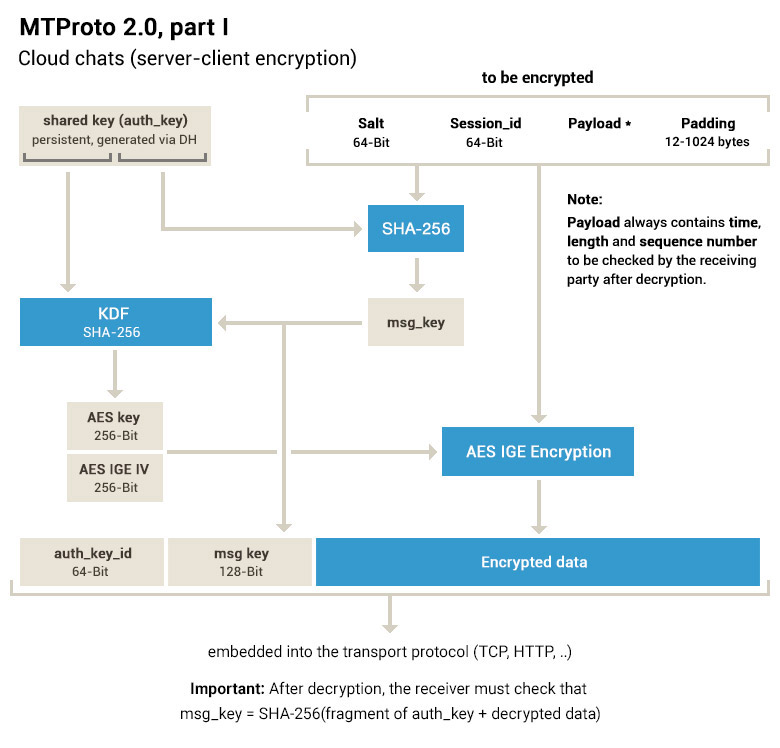
\includegraphics[width=\textwidth]{mtproto-msg-1.jpeg}
    \caption{Struttura di un messaggio con client-server encryption in \gls{mtproto} \cite{man:mtproto}} \label{fig:mtproto-message-1}
\end{figure}

\subsection{Creazione della chiave di autorizzazione}
\label{sec:auth-key}
Il primo step previsto dal protocollo è la generazione della chiave di autorizzazione.
Con questa il client è in grado di autenticarsi agli occhi del sever. \\
La procedura si conclude con un \gls{dhe}, ed è così articolata (\autoref{fig:mtproto-sequence-auth}):
\begin{enumerate}
    \item il client invia una nonce al server
    \item il server risponde con la stessa nonce, una sua nonce, un valore $pq$ calcolato come prodotto fra due numeri primi,
          ed una lista di fingerprints RSA delle chiavi pubbliche del server
    \item il client decompone $pq$ nei suoi fattori primi $p, q$
    \item il client invia al server le due nonce che identificano la sessione, i valori $p, q$ e la lista di fingerprints.
          A ciò si aggiunge una fingerprint scelta fra quelle fornite dal server, con la quale cifrare tramite RSA un payload contenente
          la serializzazione binaria dei valori $pq, p, q$, nonce, nonce del server, ed una nuova nonce generata con una randomness crittografica
    \item il server risponde con le due nonce iniziali e un payload cifrato con AES256 con chiave $t_{temp}$ realizzata a partire dalla nuova nonce segreta inviata dal client tramite \gls{kdf}.
          Il payload contiene l'hash SHA1 della nuova nonce inviata dal client,
          un numero primo $2^{2047} < N < 2^{2048} : N, \frac{p-1}{2} \in \mathbb{N}$, un generatore $g$ di un gruppo ciclico con ordine $\frac{p-1}{2}$ e il valore $g^a$,
          dove $a$ è un numero casuale generato dal server
    \item il client genera in maniera sicura un numero random $b$ di 2048 bit ed invia al server le due nonce e un crittotesto
          cifrato con la chiave temporanea ${k_temp}$ contenente il valore $g^b$
    \item da questo momento in poi la chiave di autenticazione è uguale a $g^{ab}$, che sia il server che il client sono in grado di calcolare autonomamente
    \item l'hash della chiave di autenticazione è generato a partire dai 64 bit meno significativi dell'hash SHA1 della chiave di autenticazione
    \item se tutto è andato a buon fine, il server risponderà con un messaggio di conferma. Altrimenti, con un messaggio di errore o con un invito a riprovare
\end{enumerate}

\begin{figure}
    % generated by Plantuml 1.2022.0
    \definecolor{plantucolor0000}{RGB}{255,255,255}
    \definecolor{plantucolor0001}{RGB}{56,56,56}
    \definecolor{plantucolor0002}{RGB}{248,248,248}
    \definecolor{plantucolor0003}{RGB}{0,0,0}
    \definecolor{plantucolor0004}{RGB}{235,235,235}
    \begin{tikzpicture}[xscale=0.6,yscale=-1
            ,pstyle0/.style={color=plantucolor0001,fill=white,line width=1.0pt}
            ,pstyle1/.style={color=plantucolor0001,line width=1.0pt,dash pattern=on 5.0pt off 5.0pt}
            ,pstyle2/.style={color=plantucolor0001,fill=plantucolor0002,line width=1.5pt}
            ,pstyle3/.style={color=plantucolor0001,fill=plantucolor0004,line width=1.0pt}
            ,pstyle4/.style={color=plantucolor0001,fill=plantucolor0001,line width=1.0pt}
            ,pstyle5/.style={color=plantucolor0001,line width=1.0pt}
        ]
        \draw[pstyle0] (583.0914pt,155.2pt) rectangle (593.0914pt,184.8pt);
        \draw[pstyle0] (583.0914pt,296.8001pt) rectangle (593.0914pt,393.2001pt);
        \draw[pstyle0] (583.0914pt,489.6002pt) rectangle (593.0914pt,554.8002pt);
        \draw[pstyle1] (166pt,36.7999pt) -- (166pt,572.8002pt);
        \draw[pstyle1] (587.8644pt,36.7999pt) -- (587.8644pt,572.8002pt);
        \draw[pstyle2] (139pt,5pt) rectangle (193.8pt,35.7999pt);
        \node at (134pt,12pt)[below right,color=black]{Client};
        \draw[pstyle2] (139pt,571.8002pt) rectangle (193.8pt,602.6001pt);
        \node at (134pt,578.8002pt)[below right,color=black]{Client};
        \draw[pstyle2] (559.8644pt,5pt) rectangle (616.3185pt,35.7999pt);
        \node at (555pt,12pt)[below right,color=black]{Server};
        \draw[pstyle2] (559.8644pt,571.8002pt) rectangle (616.3185pt,602.6001pt);
        \node at (555pt,578.8002pt)[below right,color=black]{Server};
        \draw[pstyle0] (583.0914pt,155.2pt) rectangle (593.0914pt,184.8pt);
        \draw[pstyle0] (583.0914pt,296.8001pt) rectangle (593.0914pt,393.2001pt);
        \draw[pstyle0] (583.0914pt,489.6002pt) rectangle (593.0914pt,554.8002pt);
        \draw[pstyle3] (113pt,51.7999pt) -- (113pt,76.7999pt) -- (218pt,76.7999pt) -- (218pt,61.7999pt) -- (208pt,51.7999pt) -- (113pt,51.7999pt);
        \draw[pstyle3] (208pt,51.7999pt) -- (208pt,61.7999pt) -- (218pt,61.7999pt) -- (208pt,51.7999pt);
        \node at (119pt,56.7999pt)[below right,color=black]{Genera $n_c$};
        \draw[pstyle3] (411pt,87.3999pt) -- (411pt,128.3999pt) -- (763pt,128.3999pt) -- (763pt,97.3999pt) -- (753pt,87.3999pt) -- (411pt,87.3999pt);
        \draw[pstyle3] (753pt,87.3999pt) -- (753pt,97.3999pt) -- (763pt,97.3999pt) -- (753pt,87.3999pt);
        \node at (417pt,92.3999pt)[below right,color=black]{Chiavi private $sk^1_s, sk^2_s, ..., sk^n_s$};
        \node at (417pt,108pt)[below right,color=black]{Genera $n_s, p, q$};
        \draw[pstyle4] (571.0914pt,151.2pt) -- (581.0914pt,155.2pt) -- (571.0914pt,159.2pt) -- (575.0914pt,155.2pt) -- cycle;
        \draw[pstyle5] (166.4pt,155.2pt) -- (577.0914pt,155.2pt);
        \node at (173.4pt,137.6pt)[below right,color=black]{$n_c$};
        \draw[pstyle4] (177.4pt,180.8pt) -- (167.4pt,184.8pt) -- (177.4pt,188.8pt) -- (173.4pt,184.8pt) -- cycle;
        \draw[pstyle5] (171.4pt,184.8pt) -- (587.0914pt,184.8pt);
        \node at (183.4pt,167.2pt)[below right,color=black]{$n_c, n_s, qp, [fp^1_s, fp^2_s, ..., fp^n_s]$};
        \draw[pstyle3] (5pt,197.8pt) -- (5pt,269.8pt) -- (327pt,269.8pt) -- (327pt,207.8pt) -- (317pt,197.8pt) -- (5pt,197.8pt);
        \draw[pstyle3] (317pt,197.8pt) -- (317pt,207.8pt) -- (327pt,207.8pt) -- (317pt,197.8pt);
        \node at (11pt,202.8pt)[below right,color=black]{Genera $n_k$};
        \node at (11pt,218.4pt)[below right,color=black]{Sceglie una chiave $pk^i_s$ fra gli $fp^i_s$};
        \node at (11pt,234pt)[below right,color=black]{Calcola $p, q, (k, iv) = \mathcal{KDF}(n_s, n_k)$};
        \node at (11pt,249.6pt)[below right,color=black]{Crea $m_1 = qp, q, p, n_c, n_k, n_s$};
        \draw[pstyle4] (571.0914pt,292.8001pt) -- (581.0914pt,296.8001pt) -- (571.0914pt,300.8001pt) -- (575.0914pt,296.8001pt) -- cycle;
        \draw[pstyle5] (166.4pt,296.8001pt) -- (577.0914pt,296.8001pt);
        \node at (173.4pt,279.2001pt)[below right,color=black]{$n_c, n_s, q, p, fp^i_s, \{\mathcal{H}(m_1), m_1\}_{pk^i_s}$};
        \draw[pstyle3] (408pt,309.8001pt) -- (408pt,365.8001pt) -- (767pt,365.8001pt) -- (767pt,319.8001pt) -- (757pt,309.8001pt) -- (408pt,309.8001pt);
        \draw[pstyle3] (757pt,309.8001pt) -- (757pt,319.8001pt) -- (767pt,319.8001pt) -- (757pt,309.8001pt);
        \node at (414pt,314.8001pt)[below right,color=black]{Genera $g, N, a \in \mathbb{Z}_P$};
        \node at (414pt,330.4001pt)[below right,color=black]{Calcola $g_a = g^a, (k, iv) = \mathcal{KDF}(n_s, n_k)$};
        \node at (414pt,346.0001pt)[below right,color=black]{Crea $m_2 = n_c, n_s, g, p, g_a, \text{time}$};
        \draw[pstyle4] (177.4pt,389.2001pt) -- (167.4pt,393.2001pt) -- (177.4pt,397.2001pt) -- (173.4pt,393.2001pt) -- cycle;
        \draw[pstyle5] (171.4pt,393.2001pt) -- (587.0914pt,393.2001pt);
        \node at (183.4pt,375.6001pt)[below right,color=black]{$n_c, n_s, \{\mathcal{H}(m_2), m_2\}_{(k, iv)}$};
        \draw[pstyle3] (25pt,406.2001pt) -- (25pt,462.2001pt) -- (306pt,462.2001pt) -- (306pt,416.2001pt) -- (296pt,406.2001pt) -- (25pt,406.2001pt);
        \draw[pstyle3] (296pt,406.2001pt) -- (296pt,416.2001pt) -- (306pt,416.2001pt) -- (296pt,406.2001pt);
        \node at (31pt,411.2001pt)[below right,color=black]{Genera $b \in \mathbb{Z}_P$};
        \node at (31pt,426.8001pt)[below right,color=black]{Calcola $k_{AS} = g^b_a \mod N$};
        \node at (31pt,442.4001pt)[below right,color=black]{Crea $m_3 = n_c, n_s, \text{retry\_id}, g_b$};
        \draw[pstyle4] (571.0914pt,485.6002pt) -- (581.0914pt,489.6002pt) -- (571.0914pt,493.6002pt) -- (575.0914pt,489.6002pt) -- cycle;
        \draw[pstyle5] (166.4pt,489.6002pt) -- (577.0914pt,489.6002pt);
        \node at (173.4pt,472.0002pt)[below right,color=black]{$n_c, n_s, \{\mathcal{H}(m_3), m_3\}_{(k, iv)}$};
        \draw[pstyle3] (471pt,502.6002pt) -- (471pt,527.6002pt) -- (704pt,527.6002pt) -- (704pt,512.6002pt) -- (694pt,502.6002pt) -- (471pt,502.6002pt);
        \draw[pstyle3] (694pt,502.6002pt) -- (694pt,512.6002pt) -- (704pt,512.6002pt) -- (694pt,502.6002pt);
        \node at (477pt,507.6002pt)[below right,color=black]{Calcola $k_{AS} = g^a_b \mod N$};
        \draw[pstyle4] (177.4pt,550.8002pt) -- (167.4pt,554.8002pt) -- (177.4pt,558.8002pt) -- (173.4pt,554.8002pt) -- cycle;
        \draw[pstyle5] (171.4pt,554.8002pt) -- (587.0914pt,554.8002pt);
        \node at (183.4pt,537.2002pt)[below right,color=black]{$n_c, n_s, \mathcal{H}(n_k)$};
    \end{tikzpicture}
    \caption{Diagramma di sequenza della creazione della chiave di autorizzazione in \gls{mtproto}.
        La funzione hash $\mathcal{H}$ è SHA1.
        $\mathcal{KDF}$ utilizza gli hash di $n_s, n_k$ per generare la chiave temporanea $k$ e il vettore di inizializzazione $iv$}. \label{fig:mtproto-sequence-auth}
\end{figure}


\subsubsection{Dettagli aggiuntivi}
Le due nonce $n_c, n_s$, generate all'inizio dello scambio di messaggi, sono integrate in tutte le comunicazioni successive,
al fine di identificare la sessione.
Si noti che il loro valore è di dominio pubblico. \\

La challenge posta con l'invio di $qp$ e la relativa fattorizzazione ha lo scopo di evitare attacchi DDos.
Un avversario che voglia minare la disponibilità del sistema dovrebbe essere in grado di svolgere un lavoro computazionale
proporzionale al numero di sessioni che si sta creando. \\
Si può parlare di questa strategia come una proof of work semplificata. \\

Il valore di retry\_id parte da 0 e diventa l'hash della chiave di autorizzazione precedente qual ora il server
richieda di rinegoziare le chiavi nella stessa sessione.
Questo può accadere, ad esempio, se l'hash della nuova chiave è già presente nella lista di hash di chiavi registrate del server. \\

Il protocollo assume che sia il client che il server verifichino la correttezza dei parametri utilizzati nelle primitive crittografiche.
Eventuali valori che non rientrano negli intervalli definiti sono scartati immediatamente, facendo fallire il protocollo.

\subsection{Chat segrete}
Oltre alla comunicazione standard con un server, il client può anche comunicare con altri client, con la garanzia che i messaggio utilizzino \gls{e2e} encryption. \\
La struttura dei messaggi è piuttosto complessa e differisce da quella riportata precedentemente (\autoref{fig:mtproto-message-2}). \\

\begin{figure}[h]
    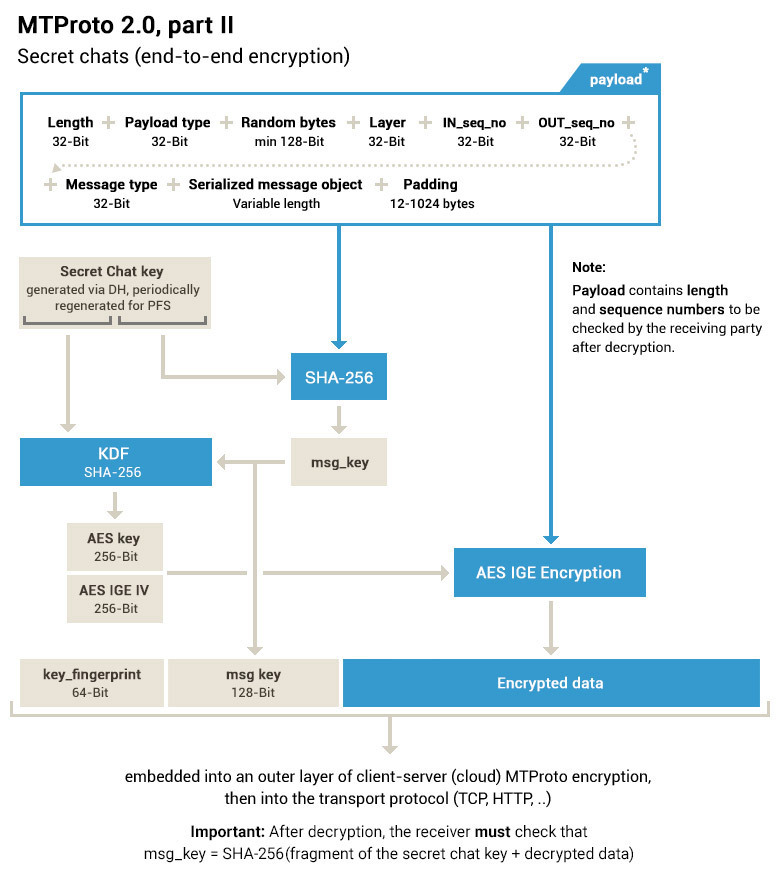
\includegraphics[width=\textwidth]{mtproto-msg-2.jpeg}
    \caption{Struttura di un messaggio con \gls{e2e} encryption in \gls{mtproto} \cite{man:mtproto}} \label{fig:mtproto-message-2}
\end{figure}

Affinché il protocollo sia in grado di garantire le proprietà di sicurezza, è necessario verificare che la chiave prodotta sia condivisa dalle due parti.
Proprio per questo l'app Telegram permette di visionare un valore prodotto dalla chiave segreta, ed invita entrambi gli utenti ad assicurarsi che entrambi vedano la stessa chiave  (\autoref{fig:encryption-key-visualization}).

\begin{figure}[h]
    \centering
    
\includegraphics{encryption-key-visualization.jpg}
    \caption{Questa schermata permette agli utenti di confrontare la chiave condivisa per l'\gls{e2e} encryption \cite{que:secret-chat}} \label{fig:encryption-key-visualization}
\end{figure}

Il setup per ottenere la chiave condivisa consiste in un \gls{dhe} e si compone dei seguenti passaggi (\autoref{fig:mtproto-sequence-secret-chat}):

\begin{enumerate}
    \item $A$ invia una richiesta al server per ricevere dei parametri $g, p$ da usare nel \gls{dhe}
    \item il server restituisce i parametri richiesti, e cifra il messaggio con la key di autenticazione $k_a$ che condivide con il server (\autoref{sec:auth-key})
    \item $A$ genera un numero casuale $a$ e produce $g_a = g^a \mod p$. Invia al server la tripla $(id, B, g_a)$, cifrata con $k_a$ dove $id$ è un identificativo di sessione
          appena generato e $B$ è il destinatario
    \item il server inoltra la richiesta, aggiungendo il mittente ed usando la chiave corretta: $\{id, B, g_a\}k_a \Rightarrow \{id, A, B, g_a\}k_b$
    \item $B$ riceve la richiesta. Se questa viene accettata, $B$ chiede al server gli stessi parametri pubblici $g, p$
    \item il server restituisce a $B$ i parametri richiesti
    \item $B$ genera un numero casuale $b$ e produce $g_b = g^b \mod p$. Calcola inoltre $k_{AB} = g_a^b$. Invia al server la tripla $(id, A, \mathcal{H}(k_{AB}))$, cifrata con $k_b$
    \item il server inoltra la richiesta modificata a dovere ad $A$
    \item $A$ calcola $k_{BA} = g_b^a$, assicurandosi che l'hash di $k_{BA}$ sia uguale a quello ricevuto nel messaggio
    \item $A$ e $B$ utilizzano un canale esterno, come l'app di Telegram, per verificare che condividono la stessa chiave
\end{enumerate}

\subsubsection{Dettagli aggiuntivi}
Tutti i messaggi che i due client scambiano con il server sono cifrati con la rispettiva chiave di autenticazione (\autoref{sec:auth-key}).
La funzione hash $\mathcal{H}$ è SHA1.
Tutti i parametri ottenuti dal server, quali $g, p, g_a \text{o} g_b$ sono controllati. Gli agenti si assicurano che rispettino determinate condizioni di sicurezza.
Nello specifico, $1 < g, g_a, g_b < p - 1$, e $2^{2048-64} < g_a, g_b < p - 2^{2048-64}$, al fine di evitare di effettuare \gls{dhe} con parametri deboli. \\


\begin{figure}
    % generated by Plantuml 1.2022.5       
    \definecolor{plantucolor0000}{RGB}{255,255,255}
    \definecolor{plantucolor0001}{RGB}{24,24,24}
    \definecolor{plantucolor0002}{RGB}{227,227,227}
    \definecolor{plantucolor0003}{RGB}{0,0,0}
    \definecolor{plantucolor0004}{RGB}{250,250,250}
    \begin{tikzpicture}[xscale=0.6,yscale=-0.85
            ,pstyle0/.style={color=plantucolor0001,fill=white,line width=1.0pt}
            ,pstyle1/.style={color=plantucolor0001,line width=0.5pt,dash pattern=on 5.0pt off 5.0pt}
            ,pstyle2/.style={color=plantucolor0001,fill=plantucolor0002,line width=0.5pt}
            ,pstyle3/.style={color=plantucolor0001,fill=plantucolor0004,line width=0.5pt}
            ,pstyle4/.style={color=plantucolor0001,fill=plantucolor0001,line width=1.0pt}
            ,pstyle5/.style={color=plantucolor0001,line width=1.0pt}
        ]
        \draw[pstyle0] (378.6934pt,179.6602pt) rectangle (388.6934pt,210.1387pt);
        \draw[pstyle0] (378.6934pt,293.5742pt) rectangle (388.6934pt,498.9238pt);
        \draw[pstyle0] (383.6934pt,354.5313pt) rectangle (393.6934pt,385.0098pt);
        \draw[pstyle0] (626.9471pt,324.0527pt) rectangle (636.9471pt,468.4453pt);
        \draw[pstyle1] (124pt,37.7461pt) -- (124pt,569.8809pt);
        \draw[pstyle1] (383.3042pt,37.7461pt) -- (383.3042pt,569.8809pt);
        \draw[pstyle1] (631.0926pt,37.7461pt) -- (631.0926pt,569.8809pt);

        \draw[pstyle2] (80pt,12pt) rectangle (180pt,36pt);
        \node at (85pt,13pt)[below right,color=black]{Client A};
        \draw[pstyle2] (80pt,575pt) rectangle (180pt,599pt);
        \node at (85pt,576pt)[below right,color=black]{Client A};

        \draw[pstyle2] (353pt,10pt) rectangle (420pt,36pt);
        \node at (355pt,13pt)[below right,color=black]{Server};
        \draw[pstyle2] (353pt,575pt) rectangle (420pt,599pt);
        \node at (355pt,576pt)[below right,color=black]{Server};

        \draw[pstyle2] (590pt,10pt) rectangle (690pt,36pt);
        \node at (595pt,13pt)[below right,color=black]{Client B};
        \draw[pstyle2] (590pt,575pt) rectangle (690pt,599pt);
        \node at (595pt,576pt)[below right,color=black]{Client B};

        \draw[pstyle0] (378.6934pt,179.6602pt) rectangle (388.6934pt,210.1387pt);
        \draw[pstyle0] (378.6934pt,293.5742pt) rectangle (388.6934pt,498.9238pt);
        \draw[pstyle0] (383.6934pt,354.5313pt) rectangle (393.6934pt,385.0098pt);
        \draw[pstyle0] (626.9471pt,324.0527pt) rectangle (636.9471pt,468.4453pt);
        \draw[pstyle3] (40pt,52.7461pt) rectangle (230pt,78.7461pt);
        \node at (46pt,57.7461pt)[below right,color=black]{Conosce la chiave $k_a$};
        \draw[pstyle3] (286pt,89.2246pt) rectangle (503pt,115.2246pt);
        \node at (292pt,94.2246pt)[below right,color=black]{Conosce le chiavi $k_a, k_b$};
        \draw[pstyle3] (547pt,125.7031pt) rectangle (738pt,151.7031pt);
        \node at (553pt,130.7031pt)[below right,color=black]{Conosce la chiave $k_b$};
        \draw[pstyle4] (366.6934pt,175.6602pt) -- (376.6934pt,179.6602pt) -- (366.6934pt,183.6602pt) -- (370.6934pt,179.6602pt) -- cycle;
        \draw[pstyle5] (124.7778pt,179.6602pt) -- (372.6934pt,179.6602pt);
        \node at (131.7778pt,161.1816pt)[below right,color=black]{$\{getDHconfig()\}k_a$};
        \draw[pstyle4] (135.7778pt,206.1387pt) -- (125.7778pt,210.1387pt) -- (135.7778pt,214.1387pt) -- (131.7778pt,210.1387pt) -- cycle;
        \draw[pstyle5] (129.7778pt,210.1387pt) -- (382.6934pt,210.1387pt);
        \node at (141.7778pt,191.6602pt)[below right,color=black]{$\{g, p\}k_a$};
        \draw[pstyle3] (5pt,223.1387pt) rectangle (245pt,265.1387pt);
        \node at (11pt,228.1387pt)[below right,color=black]{Genera $a \in \mathbb{Z}_p$ e $id$};
        \node at (11pt,244.6172pt)[below right,color=black]{Calcola $g_a = g^a \mod p$};
        \draw[pstyle4] (366.6934pt,289.5742pt) -- (376.6934pt,293.5742pt) -- (366.6934pt,297.5742pt) -- (370.6934pt,293.5742pt) -- cycle;
        \draw[pstyle5] (124.7778pt,293.5742pt) -- (372.6934pt,293.5742pt);
        \node at (131.7778pt,275.0957pt)[below right,color=black]{$\{id, B, g_a\}k_a$};
        \draw[pstyle4] (614.9471pt,320.0527pt) -- (624.9471pt,324.0527pt) -- (614.9471pt,328.0527pt) -- (618.9471pt,324.0527pt) -- cycle;
        \draw[pstyle5] (388.6934pt,324.0527pt) -- (620.9471pt,324.0527pt);
        \node at (395.6934pt,305.5742pt)[below right,color=black]{$\{id, A, B, g_a\}k_b$};
        \draw[pstyle4] (404.6934pt,350.5313pt) -- (394.6934pt,354.5313pt) -- (404.6934pt,358.5313pt) -- (400.6934pt,354.5313pt) -- cycle;
        \draw[pstyle5] (398.6934pt,354.5313pt) -- (625.9471pt,354.5313pt);
        \node at (410.6934pt,336.0527pt)[below right,color=black]{$\{chatAccepted()\}k_b$};
        \draw[pstyle4] (614.9471pt,381.0098pt) -- (624.9471pt,385.0098pt) -- (614.9471pt,389.0098pt) -- (618.9471pt,385.0098pt) -- cycle;
        \draw[pstyle5] (388.6934pt,385.0098pt) -- (620.9471pt,385.0098pt);
        \node at (395.6934pt,366.5313pt)[below right,color=black]{$\{g, p\}k_b$};
        \draw[pstyle3] (504pt,398.0098pt) rectangle (785pt,440.0098pt);
        \node at (510pt,403.0098pt)[below right,color=black]{Genera $b \in \mathbb{Z}_p$ e $id$};
        \node at (510pt,419.4883pt)[below right,color=black]{Calcola $g_b = g^b \mod p, k = g_a^b$};
        \draw[pstyle4] (399.6934pt,464.4453pt) -- (389.6934pt,468.4453pt) -- (399.6934pt,472.4453pt) -- (395.6934pt,468.4453pt) -- cycle;
        \draw[pstyle5] (393.6934pt,468.4453pt) -- (630.9471pt,468.4453pt);
        \node at (405.6934pt,449.9668pt)[below right,color=black]{$\{id, g_b, \mathcal{H}(k)\}k_b$};
        \draw[pstyle4] (135.7778pt,494.9238pt) -- (125.7778pt,498.9238pt) -- (135.7778pt,502.9238pt) -- (131.7778pt,498.9238pt) -- cycle;
        \draw[pstyle5] (129.7778pt,498.9238pt) -- (382.6934pt,498.9238pt);
        \node at (141.7778pt,480.4453pt)[below right,color=black]{$\{id, B, g_b, \mathcal{H}(k)\}k_a$};
        \draw[pstyle3] (30pt,511.9238pt) rectangle (218pt,553.9238pt);
        \node at (36pt,516.9238pt)[below right,color=black]{Calcola $k = g_b^a$};
        \node at (36pt,533.4023pt)[below right,color=black]{Controlla $\mathcal{H}(k)$};
    \end{tikzpicture}
    \caption{Diagramma di sequenza della creazione di chat segrete con crittografia \gls{e2e} in \gls{mtproto}.
        La funzione hash $\mathcal{H}$ è SHA1.} \label{fig:mtproto-sequence-secret-chat}
\end{figure}


\pagebreak

% Formal Analysis
\section{Analisi formale}

\subsection{Modello del protocollo}
Il modello del protocollo, realizzato per consentire un'analisi formale dello stesso, è realizzata con \gls{tamarin}.
Utilizzando la tecnica del \gls{multiset-rewriting}, è possibile specificare una serie di regole di riscrittura
che modellino fedelmente il comportamento degli agenti che vi partecipano. \\

In questa analisi si procederà assumendo che le primitive crittografiche utilizzate dal protocollo siano sicure.
Nello specifico, non è possibile in nessuna circostanza ottenere un testo in chiaro a partire da un testo cifrato senza conoscere la chiave,
le firme digitali non sono falsificabili e le funzioni hash sono collision-resistant. \\

Sotto queste ipotesi, ci si concentrerà sullo scambio di messaggi attraverso la rete da parte di client e server.

\subsection{Modello di attaccante}
Il modello di attaccante adottato è quello classico Dolev-Yao \cite{art:dolev-yao}. \\
In sintesi, l'attaccante ha il completo controllo del canale di comunicazione.
È quindi in grado di intercettare qualsiasi messaggio e di conoscerne il contenuto (che può essere cifrato o non),
modificarlo a piacimento e inviarlo ad un destinatario arbitrario. \\
Le uniche limitazioni imposte all'avversario sono relative alle ipotesi fatte in precedenza
sulla bontà delle primitive crittografiche, che non possono essere violate. \\

Al fine di rendere più verosimile il modello, alcuni dei server coinvolti nel protocollo potrebbero essere compromessi,
rivelando informazioni aggiuntive all'attaccante.

\subsection{Proprietà di sicurezza}
Ogni sottosezione di \gls{mtproto} soddisfa uno specifico obiettivo.
Nel complesso, l'intero protocollo dovrebbe garantire le seguenti proprietà:
\begin{itemize}
    \item \textbf{Secrecy:} se un messaggio $m$ viene scambiato fra due agenti onesti $A$, $B$ durante una session $S$,
          il contenuto del messaggio è noto solo ad $A$ e $B$
    \item \textbf{Forward secrecy:} una chiave di sessione $s$ non viene compromessa
          anche se la chiave a lungo termine usata per generarla viene compromessa
    \item \textbf{Authentication:} se $B$ riceve un messaggio che, seguendo il protocollo,
          attribuisce ad $A$, questo è stato effettivamente inviato da $A$
    \item \textbf{Integrity:} se $A$ invia un messaggio $m$ a $B$
          e questo riceve un messaggio $m'$ da $A$, ne segue che $m' = m$
\end{itemize}

\subsection{Authorization key protocol}
La verifica del protocollo di creazione dell'Authorization Key dimostra in maniera formale le proprietà di sicurezza attese.

\subsubsection{Authentication}

\begin{lstlisting}[caption=Il client non è autenticato agli occhi del server.
    Anche un avversario può iniziare legittimamente il protocollo. Questo lemma è falso.,
    label=cod:lemma:client_auth]
lemma client_auth:
    "
    All nc ns pkS #i .
        // Se S accetta l'inizio del protocollo...
        S_AcceptStart(nc, ns, pkS) @ i
        ==>
        Ex #j . 
            // ... C ha mandato il primo messaggio
            C_Start(nc) @ j
            & j < i
    "
\end{lstlisting}

\begin{lstlisting}[caption={Se il client ha ricevuto i parametri relativi a DHE, è stato il server ad inviarli.},
    label=cod:lemma:auth_dh]
lemma auth_dh:
    "
    All nc ns nk N ga tk #i .
        // Se C ha ricevuto i parametri relativi a DHE,
        // che ha decifrato con tk...
        C_ReceivesDHParameters(nc, ns, N, ga) @ i
        & C_GenerateTK(nc, ns, nk, tk) @ i
        ==>
        ( Ex #j .
            // ... li ha inviati S...
            S_SendsDHParameters(nc, ns, N, ga) @ j
            & j < i
        )
        | // ... a meno che non sia stato rivelato skS o nk
        ( Ex skS #k .
            RevealSkS(skS) @k
        )
        |
        ( Ex #k .
            RevealNK(nk) @k
        )
    "
\end{lstlisting}

\begin{lstlisting}[caption={Se il protocollo si è concluso con successo, il client e il server hanno entrambi portato 
    a termine il protollo},
    label=cod:lemma:success_auth]
lemma success_auth:
    "
    All nc ns nk kas #i .
        // Se C ha completato con successo il protocollo, ottenendo kas...
        C_Success(nc, ns, kas) @ i
        & C_SuccessSecrets(nc, ns, nk) @ i
        ==>
        ( Ex #j .
            // ... anche S ha raggiunto la stessa conclusione
            S_Success(nc, ns, kas) @ j
            & j < i
        )
        | // ... a meno che non sia stato rivelato skS o nk
        ( Ex skS #k .
            RevealSkS(skS) @k
        )
        |
        ( Ex #k .
            RevealNK(nk) @k
        )
    "
\end{lstlisting}

\subsubsection{Secrecy e Forward Secrecy}

\begin{lstlisting}[caption={Se la chiave privata del server non è compromessa e non è rivelata per errore,
    l'avversario non arriva a conoscere la nonce nk condivisa
    fra C ed S.},
    label=cod:lemma:secret_nk]
lemma secret_nk:
    "
    All nc ns nk #i .
        // Se C genera nk...
        C_GenerateNK(nc, ns, nk) @ i
        ==> 
        // ... l'avversario non ha modo di conoscere il suo valore
        ( not   ( Ex #k .
                    K(nk) @ k
                )
        )
        | // ... a meno che non sia stato rivelato skS o nk
        ( Ex skS #k .
            RevealSkS(skS) @k
        )
        | 
        ( Ex #k .
            RevealNK(nk) @k
        )
    "
\end{lstlisting}

\begin{lstlisting}[caption={Se il client e il server hanno ottenuto una chiave condivisa kas,
    sono i soli a conoscerla.},
    label=cod:lemma:secret_kas]
lemma secret_kas:
    "
    All nc ns nk kas #i .
        // Se C ha completato con successo il protocollo, ottenendo kas...
        C_Success(nc, ns, kas) @ i
        & C_SuccessSecrets(nc, ns, nk) @ i
        ==> 
        // ... un attaccante non ha modo di conoscere kas
        ( not ( Ex #k .
                K(kas) @ k
            )
        )
        | // ... a meno che non sia stato rivelato skS o nk
        ( Ex skS #k .
            RevealSkS(skS) @k
        )
        |
        ( Ex #k .
            RevealNK(nk) @k
        )
    "
\end{lstlisting}

\begin{lstlisting}[caption={Se il client e il server hanno ottenuto una chiave condivisa kas,
    sono i soli a conoscerla.
    Questa rimane sicura anche se avvengono dei leak a posteriori di informazioni segrete,
    garantendo forward secrecy, purchè ciò avvenga dopo il quarto messaggio del protocollo.},
    label=cod:lemma:secret_kas_leaks]
lemma secret_kas_leaks:
    "
    All nc ns nk tk kas #i .
        // Se C ha generato kas...
        C_CreateKas(nc, ns, kas) @ i
        & C_GenerateTK(nc, ns, nk, tk) @ i
        ==> 
        // ... un attaccante non ha modo di conoscere kas
        not ( Ex #k .
                K(kas) @ k
            )
        | // ... a meno che non sia stato rivelato skS o nk prima del quarto messaggio
        ( Ex skS #k .
            RevealSkS(skS) @k
            & k < i
        )
        |
        ( Ex #k .
            RevealNK(nk) @k
            & k < i
        )
    "
\end{lstlisting}

\subsubsection{Integrity}

\begin{lstlisting}[caption={Se il client e il server hanno ottenuto una chiave condivisa kas nella 
    stessa sessione, questa è uguale per entrambi},
    label=cod:lemma:agreement_kas]
lemma agreement_kas:
    "
    All nc ns nk c_kas s_kas #i #j .
        // Se C e S hanno completato con successo il protocollo, ottenendo c_kas e s_kas...
        C_Success(nc, ns, c_kas) @ i
        & C_SuccessSecrets(nc, ns, nk) @ i
        & S_Success(nc, ns, s_kas) @ j
        ==>
        // ... le due chiavi ottenute coincidono
        c_kas = s_kas
        | // ... a meno che non sia stato rivelato skS o nk
        ( Ex skS #k .
            RevealSkS(skS) @k
        )
        |
        ( Ex #k .
            RevealNK(nk) @k
        )
    "
\end{lstlisting}

\begin{lstlisting}[caption={Se il client e il server hanno ottenuto una stessa chiave condivisa kas,
    è perchè stanno partecipendo alla medesima sessione},
    label=cod:lemma:agreement_session]
lemma agreement_session:
    "
    All c_nc c_ns s_nc s_ns nk kas #i #j .
        // Se C e S hanno ottenuto la stessa chiave kas...
        C_Success(c_nc, c_ns, kas) @ i
        & C_SuccessSecrets(c_nc, c_ns, nk) @ i
        & S_Success(s_nc, s_ns, kas) @ j
        ==>
        // ... partecipavano allo stesso protocollo
        c_nc = s_nc & c_ns = s_ns
        | // ... a meno che non sia stato rivelato skS o nk
        ( Ex skS #k .
            RevealSkS(skS) @k
        )
        |
        ( Ex #k .
            RevealNK(nk) @k
        )
    "
\end{lstlisting}
\pagebreak

% Formal Analysis
\section{Conclusione}
L'analisi formale effettuata con \gls{tamarin} rappresenta un'ulteriore conferma della bontà del protocollo \gls{mtproto}.
I risultati ricalcano fedelmente quelli ottenuti dall'analisi formale realizzata con ProVerif \cite{book:proverif} \cite{inp:mtproto-proverif}. \\

Si noti tuttavia che le normali chat di Telegram non presentano cifratura \gls{e2e}, e sono quindi consultabili da chi ottenga la chiave di autenticazione
a lungo termine. Ciò include il server. \\
Al contrario, le chat segrete realizzano un canale di comunicazione in grado di garantire la segretezza dei messaggi, a patto che gli utenti abbiano
l'accortezza di verificare che il protocollo sia andato a buon fine consultando vicendevolmente l'apposita schermata dell'app.
\pagebreak

% Bibliography
\printglossary
\pagebreak
\printbibliography
\pagebreak

\begin{appendices}

    \section{Implementazione in Tamarin}
    \subsection{Authorization key protocol}
    \lstinputlisting[caption=Implementazione completa della verifica formale dell'Authorization key protocol realizzata in tamarin.,
        label=cod:tamarin-auth-key]{../mtproto/MTProto_AuthKey_Creation.spthy}

    \subsection{Secret chat protocol}
    \lstinputlisting[caption=Implementazione completa della verifica formale delle Secret chat protocol realizzata in tamarin.,
        label=cod:tamarin-secret-chat]{../mtproto/MTProto_Secret_Chat.spthy}

\end{appendices}

\end{document}